\documentclass{extbook}[14pt]
\usepackage{multicol, enumerate, enumitem, hyperref, color, soul, setspace, parskip, fancyhdr, amssymb, amsthm, amsmath, bbm, latexsym, units, mathtools}
\everymath{\displaystyle}
\usepackage[headsep=0.5cm,headheight=0cm, left=1 in,right= 1 in,top= 1 in,bottom= 1 in]{geometry}
\usepackage{dashrule}  % Package to use the command below to create lines between items
\newcommand{\litem}[1]{\item #1

\rule{\textwidth}{0.4pt}}
\pagestyle{fancy}
\lhead{}
\chead{Answer Key for Progress Quiz 9 Version C}
\rhead{}
\lfoot{8590-6105}
\cfoot{}
\rfoot{Fall 2020}
\begin{document}
\textbf{This key should allow you to understand why you choose the option you did (beyond just getting a question right or wrong). \href{https://xronos.clas.ufl.edu/mac1105spring2020/courseDescriptionAndMisc/Exams/LearningFromResults}{More instructions on how to use this key can be found here}.}

\textbf{If you have a suggestion to make the keys better, \href{https://forms.gle/CZkbZmPbC9XALEE88}{please fill out the short survey here}.}

\textit{Note: This key is auto-generated and may contain issues and/or errors. The keys are reviewed after each exam to ensure grading is done accurately. If there are issues (like duplicate options), they are noted in the offline gradebook. The keys are a work-in-progress to give students as many resources to improve as possible.}

\rule{\textwidth}{0.4pt}

\begin{enumerate}\litem{
Describe the end behavior of the polynomial below.
\[ f(x) = -6(x + 4)^{5}(x - 4)^{10}(x + 8)^{2}(x - 8)^{2} \]

The solution is the graph below, which is option A.
\begin{center}
    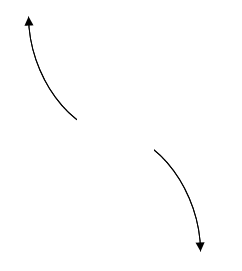
\includegraphics[width=0.3\textwidth]{../Figures/polyEndBehaviorAC.png}
\end{center}\begin{enumerate}[label=\Alph*.]
\begin{multicols}{2}
\item 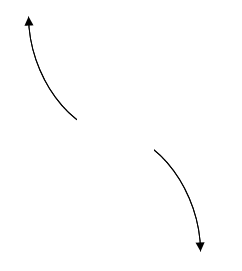
\includegraphics[width = 0.3\textwidth]{../Figures/polyEndBehaviorAC.png}
\item 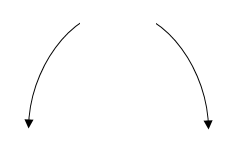
\includegraphics[width = 0.3\textwidth]{../Figures/polyEndBehaviorBC.png}
\item 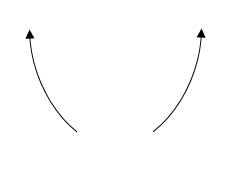
\includegraphics[width = 0.3\textwidth]{../Figures/polyEndBehaviorCC.png}
\item 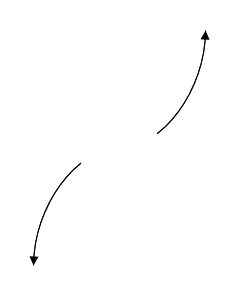
\includegraphics[width = 0.3\textwidth]{../Figures/polyEndBehaviorDC.png}
\end{multicols}\item None of the above.\end{enumerate}
\textbf{General Comment:} Remember that end behavior is determined by the leading coefficient AND whether the \textbf{sum} of the multiplicities is positive or negative.
}
\litem{
Which of the following equations \textit{could} be of the graph presented below?

\begin{center}
    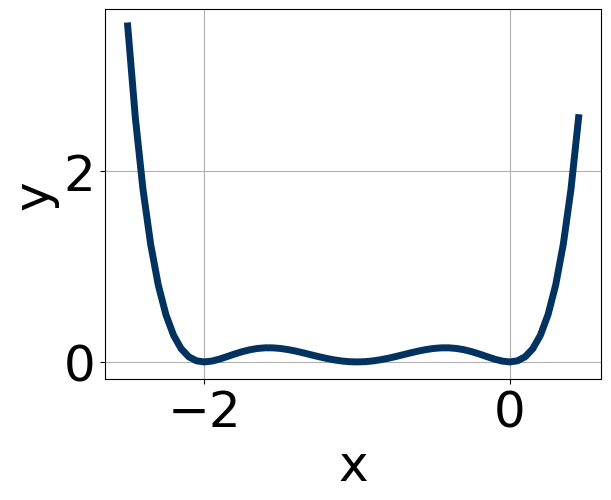
\includegraphics[width=0.5\textwidth]{../Figures/polyGraphToFunctionCopyC.png}
\end{center}




The solution is \( 18x^{8} (x + 1)^{8} (x + 2)^{8} \), which is option E.\begin{enumerate}[label=\Alph*.]
\item \( -3x^{4} (x + 1)^{8} (x + 2)^{7} \)

The factor $(x + 2)$ should have an even power and the leading coefficient should be the opposite sign.
\item \( 3x^{10} (x + 1)^{9} (x + 2)^{9} \)

The factors $(x + 1)$ and $(x + 2)$ should both have even powers.
\item \( -10x^{6} (x + 1)^{6} (x + 2)^{8} \)

This corresponds to the leading coefficient being the opposite value than it should be.
\item \( 14x^{8} (x + 1)^{10} (x + 2)^{5} \)

The factor $(x + 2)$ should have an even power.
\item \( 18x^{8} (x + 1)^{8} (x + 2)^{8} \)

* This is the correct option.
\end{enumerate}

\textbf{General Comment:} General Comments: Draw the x-axis to determine which zeros are touching (and so have even multiplicity) or cross (and have odd multiplicity).
}
\litem{
Construct the lowest-degree polynomial given the zeros below. Then, choose the intervals that contain the coefficients of the polynomial in the form $ax^3+bx^2+cx+d$.
\[ \frac{1}{4}, \frac{-1}{5}, \text{ and } \frac{1}{2} \]

The solution is \( 40x^{3} -22 x^{2} -x + 1 \), which is option A.\begin{enumerate}[label=\Alph*.]
\item \( a \in [38, 42], b \in [-22.1, -20.7], c \in [-1.03, 0.65], \text{ and } d \in [0.99, 2.17] \)

* $40x^{3} -22 x^{2} -x + 1$, which is the correct option.
\item \( a \in [38, 42], b \in [-6.3, -1.7], c \in [-8.44, -6.66], \text{ and } d \in [-2.34, -0.38] \)

$40x^{3} -2 x^{2} -7 x -1$, which corresponds to multiplying out $(4x + 1)(5x + 1)(2x -1)$.
\item \( a \in [38, 42], b \in [-18.8, -14.4], c \in [-4.18, -1.92], \text{ and } d \in [0.99, 2.17] \)

$40x^{3} -18 x^{2} -3 x + 1$, which corresponds to multiplying out $(4x + 1)(5x -1)(2x -1)$.
\item \( a \in [38, 42], b \in [19.4, 22.1], c \in [-1.03, 0.65], \text{ and } d \in [-2.34, -0.38] \)

$40x^{3} +22 x^{2} -x -1$, which corresponds to multiplying out $(4x + 1)(5x -1)(2x + 1)$.
\item \( a \in [38, 42], b \in [-22.1, -20.7], c \in [-1.03, 0.65], \text{ and } d \in [-2.34, -0.38] \)

$40x^{3} -22 x^{2} -x -1$, which corresponds to multiplying everything correctly except the constant term.
\end{enumerate}

\textbf{General Comment:} To construct the lowest-degree polynomial, you want to multiply out $(4x -1)(5x + 1)(2x -1)$
}
\litem{
Construct the lowest-degree polynomial given the zeros below. Then, choose the intervals that contain the coefficients of the polynomial in the form $ax^3+bx^2+cx+d$.
\[ \frac{1}{4}, \frac{-7}{3}, \text{ and } \frac{3}{4} \]

The solution is \( 48x^{3} +64 x^{2} -103 x + 21 \), which is option C.\begin{enumerate}[label=\Alph*.]
\item \( a \in [48, 52], b \in [61, 71], c \in [-104, -99], \text{ and } d \in [-22, -14] \)

$48x^{3} +64 x^{2} -103 x -21$, which corresponds to multiplying everything correctly except the constant term.
\item \( a \in [48, 52], b \in [83, 93], c \in [-72, -63], \text{ and } d \in [-22, -14] \)

$48x^{3} +88 x^{2} -65 x -21$, which corresponds to multiplying out $(4x + 1)(3x + 7)(4x -3)$.
\item \( a \in [48, 52], b \in [61, 71], c \in [-104, -99], \text{ and } d \in [19, 28] \)

* $48x^{3} +64 x^{2} -103 x + 21$, which is the correct option.
\item \( a \in [48, 52], b \in [-65, -63], c \in [-104, -99], \text{ and } d \in [-22, -14] \)

$48x^{3} -64 x^{2} -103 x -21$, which corresponds to multiplying out $(4x + 1)(3x -7)(4x + 3)$.
\item \( a \in [48, 52], b \in [-144, -132], c \in [38, 50], \text{ and } d \in [19, 28] \)

$48x^{3} -136 x^{2} +47 x + 21$, which corresponds to multiplying out $(4x + 1)(3x -7)(4x -3)$.
\end{enumerate}

\textbf{General Comment:} To construct the lowest-degree polynomial, you want to multiply out $(4x -1)(3x + 7)(4x -3)$
}
\litem{
Construct the lowest-degree polynomial given the zeros below. Then, choose the intervals that contain the coefficients of the polynomial in the form $x^3+bx^2+cx+d$.
\[ 3 + 4 i \text{ and } -1 \]

The solution is \( x^{3} -5 x^{2} +19 x + 25 \), which is option A.\begin{enumerate}[label=\Alph*.]
\item \( b \in [-7, -4], c \in [18.23, 21.41], \text{ and } d \in [23.7, 26.32] \)

* $x^{3} -5 x^{2} +19 x + 25$, which is the correct option.
\item \( b \in [1, 3], c \in [-2.11, -1.71], \text{ and } d \in [-3.94, -2.28] \)

$x^{3} + x^{2} -2 x -3$, which corresponds to multiplying out $(x -3)(x + 1)$.
\item \( b \in [1, 3], c \in [-3.03, -2.44], \text{ and } d \in [-6.22, -3.95] \)

$x^{3} + x^{2} -3 x -4$, which corresponds to multiplying out $(x -4)(x + 1)$.
\item \( b \in [3, 17], c \in [18.23, 21.41], \text{ and } d \in [-25.16, -24.62] \)

$x^{3} +5 x^{2} +19 x -25$, which corresponds to multiplying out $(x-(3 + 4 i))(x-(3 - 4 i))(x -1)$.
\item \( \text{None of the above.} \)

This corresponds to making an unanticipated error or not understanding how to use nonreal complex numbers to create the lowest-degree polynomial. If you chose this and are not sure what you did wrong, please contact the coordinator for help.
\end{enumerate}

\textbf{General Comment:} Remember that the conjugate of $a+bi$ is $a-bi$. Since these zeros always come in pairs, we need to multiply out $(x-(3 + 4 i))(x-(3 - 4 i))(x-(-1))$.
}
\litem{
Construct the lowest-degree polynomial given the zeros below. Then, choose the intervals that contain the coefficients of the polynomial in the form $x^3+bx^2+cx+d$.
\[ -3 - 2 i \text{ and } -3 \]

The solution is \( x^{3} +9 x^{2} +31 x + 39 \), which is option D.\begin{enumerate}[label=\Alph*.]
\item \( b \in [-13, -6], c \in [30.93, 31.32], \text{ and } d \in [-42.1, -37.4] \)

$x^{3} -9 x^{2} +31 x -39$, which corresponds to multiplying out $(x-(-3 - 2 i))(x-(-3 + 2 i))(x -3)$.
\item \( b \in [-7, 3], c \in [5.16, 6.14], \text{ and } d \in [8.1, 9.3] \)

$x^{3} + x^{2} +6 x + 9$, which corresponds to multiplying out $(x + 3)(x + 3)$.
\item \( b \in [-7, 3], c \in [4.11, 5.57], \text{ and } d \in [3.2, 8.6] \)

$x^{3} + x^{2} +5 x + 6$, which corresponds to multiplying out $(x + 2)(x + 3)$.
\item \( b \in [7, 11], c \in [30.93, 31.32], \text{ and } d \in [38.3, 41.1] \)

* $x^{3} +9 x^{2} +31 x + 39$, which is the correct option.
\item \( \text{None of the above.} \)

This corresponds to making an unanticipated error or not understanding how to use nonreal complex numbers to create the lowest-degree polynomial. If you chose this and are not sure what you did wrong, please contact the coordinator for help.
\end{enumerate}

\textbf{General Comment:} Remember that the conjugate of $a+bi$ is $a-bi$. Since these zeros always come in pairs, we need to multiply out $(x-(-3 - 2 i))(x-(-3 + 2 i))(x-(-3))$.
}
\litem{
Describe the zero behavior of the zero $x = 9$ of the polynomial below.
\[ f(x) = -7(x - 8)^{4}(x + 8)^{3}(x - 9)^{11}(x + 9)^{8} \]

The solution is the graph below, which is option A.
\begin{center}
    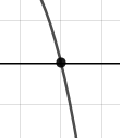
\includegraphics[width=0.3\textwidth]{../Figures/polyZeroBehaviorCopyAC.png}
\end{center}\begin{enumerate}[label=\Alph*.]
\begin{multicols}{2}
\item 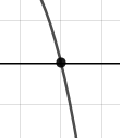
\includegraphics[width = 0.3\textwidth]{../Figures/polyZeroBehaviorCopyAC.png}
\item 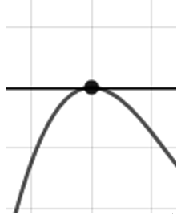
\includegraphics[width = 0.3\textwidth]{../Figures/polyZeroBehaviorCopyBC.png}
\item 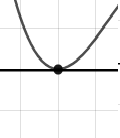
\includegraphics[width = 0.3\textwidth]{../Figures/polyZeroBehaviorCopyCC.png}
\item 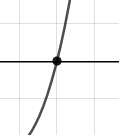
\includegraphics[width = 0.3\textwidth]{../Figures/polyZeroBehaviorCopyDC.png}
\end{multicols}\item None of the above.\end{enumerate}
\textbf{General Comment:} You will need to sketch the entire graph, then zoom in on the zero the question asks about.
}
\litem{
Describe the end behavior of the polynomial below.
\[ f(x) = 8(x - 4)^{5}(x + 4)^{8}(x + 5)^{2}(x - 5)^{4} \]

The solution is the graph below, which is option D.
\begin{center}
    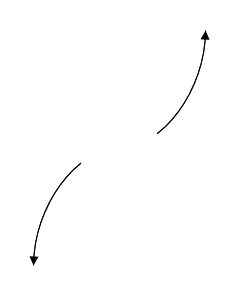
\includegraphics[width=0.3\textwidth]{../Figures/polyEndBehaviorCopyDC.png}
\end{center}\begin{enumerate}[label=\Alph*.]
\begin{multicols}{2}
\item 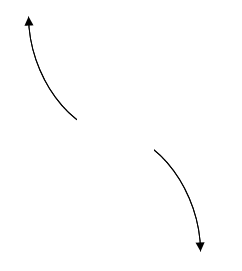
\includegraphics[width = 0.3\textwidth]{../Figures/polyEndBehaviorCopyAC.png}
\item 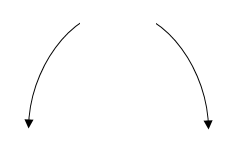
\includegraphics[width = 0.3\textwidth]{../Figures/polyEndBehaviorCopyBC.png}
\item 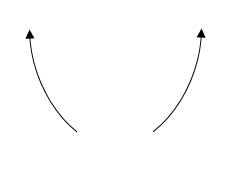
\includegraphics[width = 0.3\textwidth]{../Figures/polyEndBehaviorCopyCC.png}
\item 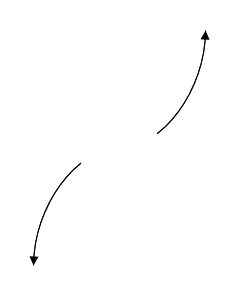
\includegraphics[width = 0.3\textwidth]{../Figures/polyEndBehaviorCopyDC.png}
\end{multicols}\item None of the above.\end{enumerate}
\textbf{General Comment:} Remember that end behavior is determined by the leading coefficient AND whether the \textbf{sum} of the multiplicities is positive or negative.
}
\litem{
Which of the following equations \textit{could} be of the graph presented below?

\begin{center}
    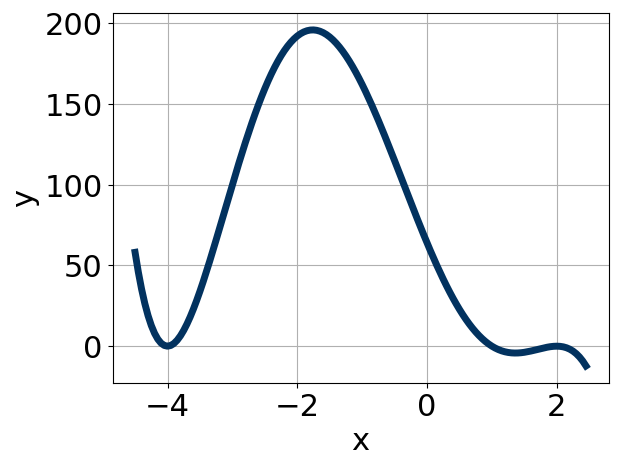
\includegraphics[width=0.5\textwidth]{../Figures/polyGraphToFunctionC.png}
\end{center}




The solution is \( 3(x - 2)^{11} (x - 3)^{5} (x + 2)^{11} \), which is option E.\begin{enumerate}[label=\Alph*.]
\item \( -16(x - 2)^{8} (x - 3)^{5} (x + 2)^{7} \)

The factor $(x - 2)$ should have an odd power and the leading coefficient should be the opposite sign.
\item \( -2(x - 2)^{7} (x - 3)^{9} (x + 2)^{7} \)

This corresponds to the leading coefficient being the opposite value than it should be.
\item \( 2(x - 2)^{10} (x - 3)^{8} (x + 2)^{9} \)

The factors $2$ and $3$ have have been odd power.
\item \( 6(x - 2)^{4} (x - 3)^{5} (x + 2)^{9} \)

The factor $2$ should have been an odd power.
\item \( 3(x - 2)^{11} (x - 3)^{5} (x + 2)^{11} \)

* This is the correct option.
\end{enumerate}

\textbf{General Comment:} General Comments: Draw the x-axis to determine which zeros are touching (and so have even multiplicity) or cross (and have odd multiplicity).
}
\litem{
Describe the zero behavior of the zero $x = 7$ of the polynomial below.
\[ f(x) = -5(x + 7)^{9}(x - 7)^{14}(x - 9)^{5}(x + 9)^{6} \]

The solution is the graph below, which is option C.
\begin{center}
    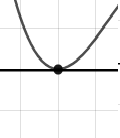
\includegraphics[width=0.3\textwidth]{../Figures/polyZeroBehaviorCC.png}
\end{center}\begin{enumerate}[label=\Alph*.]
\begin{multicols}{2}
\item 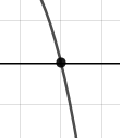
\includegraphics[width = 0.3\textwidth]{../Figures/polyZeroBehaviorAC.png}
\item 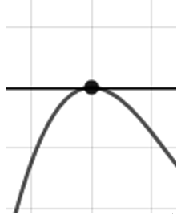
\includegraphics[width = 0.3\textwidth]{../Figures/polyZeroBehaviorBC.png}
\item 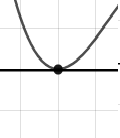
\includegraphics[width = 0.3\textwidth]{../Figures/polyZeroBehaviorCC.png}
\item 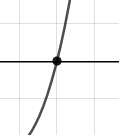
\includegraphics[width = 0.3\textwidth]{../Figures/polyZeroBehaviorDC.png}
\end{multicols}\item None of the above.\end{enumerate}
\textbf{General Comment:} You will need to sketch the entire graph, then zoom in on the zero the question asks about.
}
\end{enumerate}

\end{document}